\documentclass[11pt]{standalone}
\usepackage{tikz}        % Графический пакет tikz
\usepackage{pgfplots}
\pgfplotsset{width=10cm,compat=1.9} % Графики
\usepackage{tikz-cd}     % Коммутативные диаграммы
\usepackage{tkz-euclide} % Геометрия
\usepackage{stackengine} % Многострочные тексты в картинках
\usetikzlibrary{patterns}
\usetikzlibrary{angles, babel, quotes}

\begin{document}
	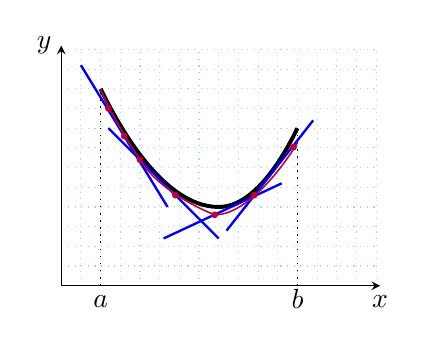
\begin{tikzpicture}[>=stealth]
		% Рисуем сетку
		\draw[help lines, step=0.25, dotted]
		(0,0) grid (4,3);
		% Начало координат
		\draw[->, thin] (0,0) -- (4.05,0)
		node[below] {$x$}; % Ox
		\draw[->, thin] (0,0) -- (0, 3.05)
		node[left] {$y$}; % Oy
		
		\draw[line width =.02cm, dotted] (0.5, 0) -- (0.5, 2.5);
		\draw[line width =.02cm, dotted] (3, 0) -- (3, 2);
		
		\draw[line width =.05cm](0.5, 2.5) parabola bend (2, 1)(3, 2);
		
		\draw[line width =.03cm, blue] (0.25, 2.8) -- (1.35, 1);
		\draw[line width =.03cm, blue] (0.6, 2) -- (2, 0.6);
		\draw[line width =.03cm, blue] (1.3, 0.6) -- (2.8, 1.3);
		\draw[line width =.03cm, blue] (2.1, 0.7) -- (3.2, 2.1);	
		
		\draw [fill = purple,purple] (0.6,2.25) circle (1pt);
		\draw [fill = purple,purple] (0.8,1.9) circle (1pt);
		\draw [fill = purple,purple] (1,1.6) circle (1pt);
		\draw [fill = purple,purple] (1.45,1.15) circle (1pt);
		\draw [fill = purple,purple] (1.95,0.9) circle (1pt);
		\draw [fill = purple,purple] (2.45,1.15) circle (1pt);	
		\draw [fill = purple,purple] (2.95,1.76) circle (1pt);
								
		\draw[line width =.02cm, purple] (0.5, 2.5).. controls (0.6,2.25) and (0.8,1.9) .. (1,1.6);
		\draw[line width =.02cm, purple] (1,1.6) .. controls (1.28,1.15) and (1.95,0.9) .. (1.95,0.9);
		\draw[line width =.02cm, purple] (1.95,0.9) .. controls (2.45,0.9) and (3,1.8) .. (3,1.82);
		
		\node[below] at (0.5, 0) {$a$};
		\node[below] at (3, 0.085) {$b$};
		
		
	\end{tikzpicture}
\end{document}
